% Created by tikzDevice version 0.12.6 on 2025-01-17 13:26:18
% !TEX encoding = UTF-8 Unicode
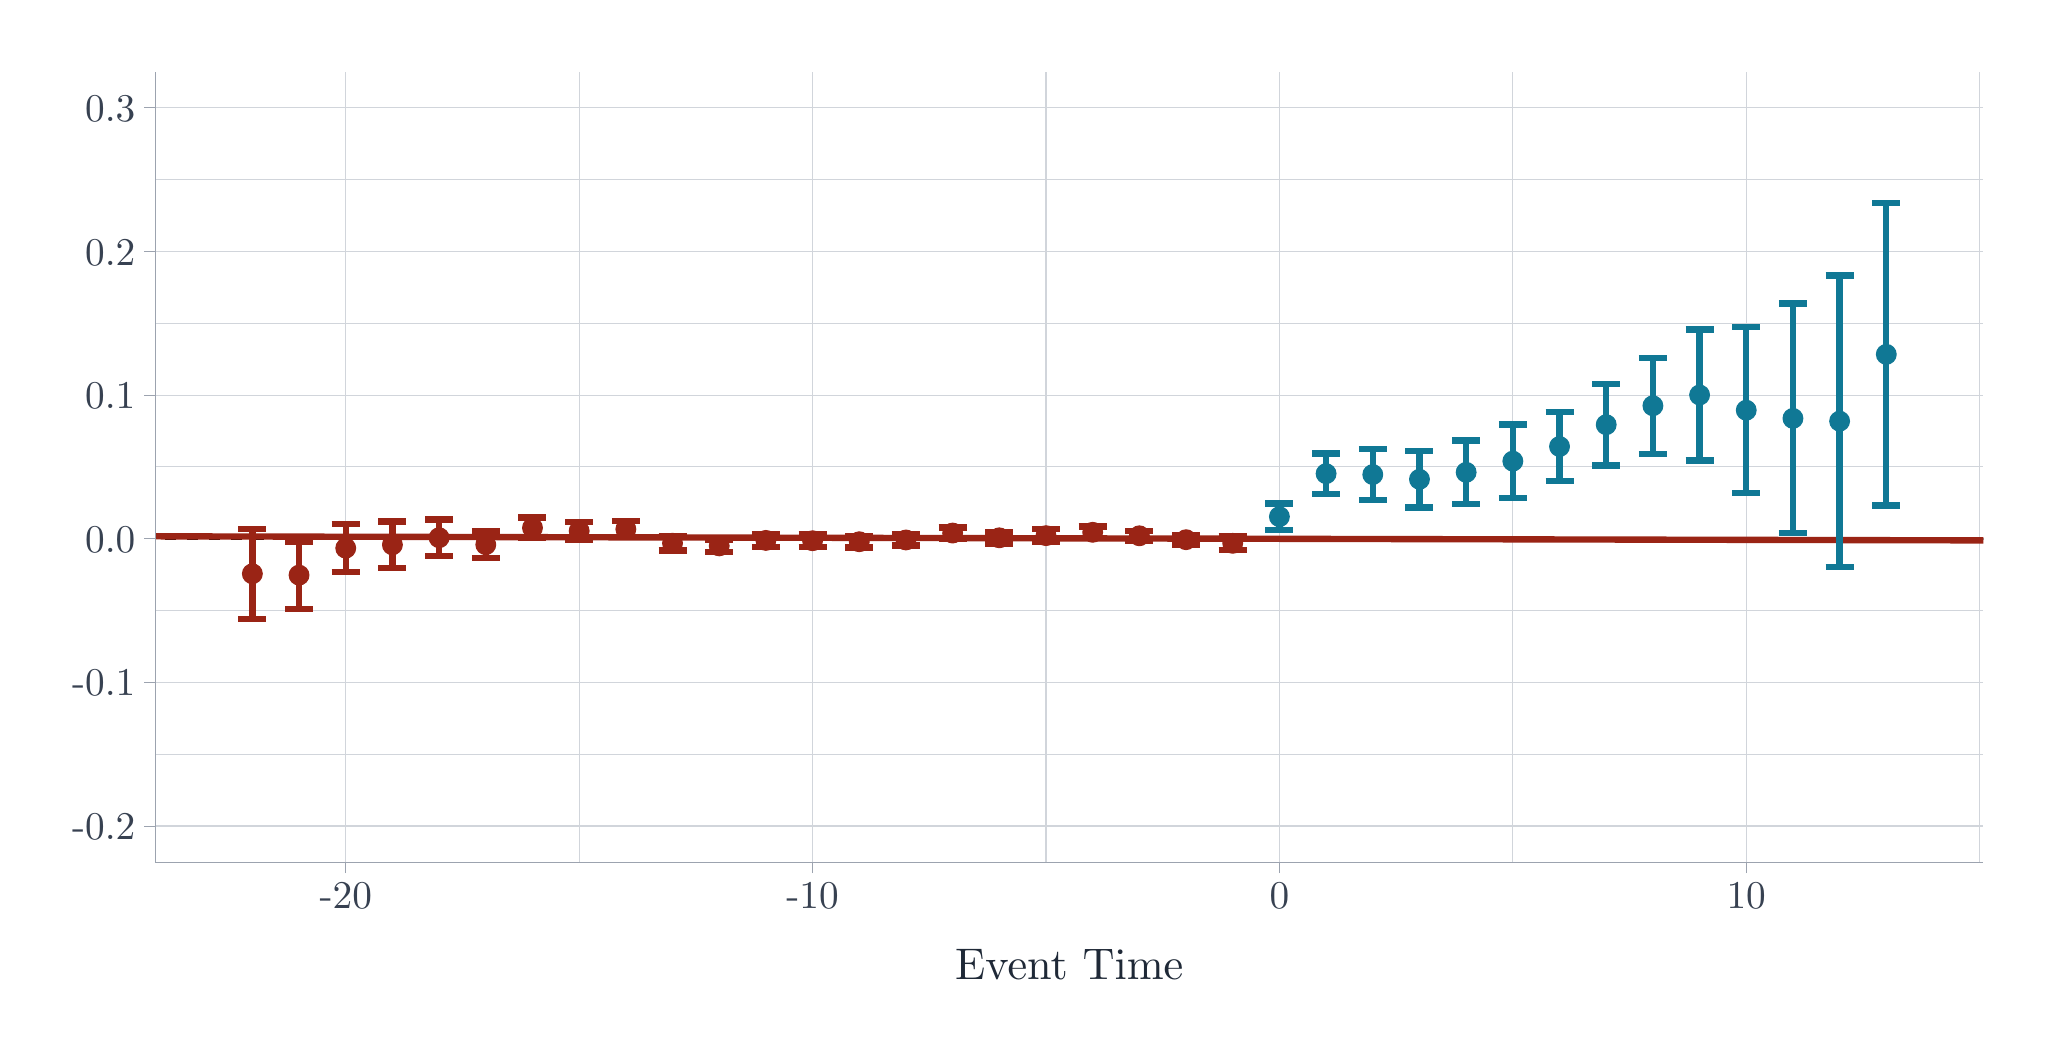
\begin{tikzpicture}[x=1pt,y=1pt]
\definecolor{fillColor}{RGB}{255,255,255}
\path[use as bounding box,fill=fillColor] (0,0) rectangle (722.70,361.35);
\begin{scope}
\path[clip] (  0.00,  0.00) rectangle (722.70,361.35);
\definecolor{drawColor}{RGB}{255,255,255}

\path[draw=drawColor,line width= 0.8pt,line join=round,line cap=round,fill=fillColor] (  0.00,  0.00) rectangle (722.70,361.35);
\end{scope}
\begin{scope}
\path[clip] ( 46.10, 59.89) rectangle (706.70,345.35);
\definecolor{drawColor}{RGB}{255,255,255}
\definecolor{fillColor}{RGB}{255,255,255}

\path[draw=drawColor,line width= 0.8pt,line join=round,line cap=round,fill=fillColor] ( 46.10, 59.89) rectangle (706.70,345.35);
\definecolor{drawColor}{RGB}{209,213,219}

\path[draw=drawColor,line width= 0.4pt,line join=round] ( 46.10, 98.81) --
	(706.70, 98.81);

\path[draw=drawColor,line width= 0.4pt,line join=round] ( 46.10,150.72) --
	(706.70,150.72);

\path[draw=drawColor,line width= 0.4pt,line join=round] ( 46.10,202.62) --
	(706.70,202.62);

\path[draw=drawColor,line width= 0.4pt,line join=round] ( 46.10,254.52) --
	(706.70,254.52);

\path[draw=drawColor,line width= 0.4pt,line join=round] ( 46.10,306.42) --
	(706.70,306.42);

\path[draw=drawColor,line width= 0.4pt,line join=round] (199.28, 59.89) --
	(199.28,345.35);

\path[draw=drawColor,line width= 0.4pt,line join=round] (367.97, 59.89) --
	(367.97,345.35);

\path[draw=drawColor,line width= 0.4pt,line join=round] (536.66, 59.89) --
	(536.66,345.35);

\path[draw=drawColor,line width= 0.4pt,line join=round] (705.35, 59.89) --
	(705.35,345.35);

\path[draw=drawColor,line width= 0.4pt,line join=round] ( 46.10, 72.86) --
	(706.70, 72.86);

\path[draw=drawColor,line width= 0.4pt,line join=round] ( 46.10,124.77) --
	(706.70,124.77);

\path[draw=drawColor,line width= 0.4pt,line join=round] ( 46.10,176.67) --
	(706.70,176.67);

\path[draw=drawColor,line width= 0.4pt,line join=round] ( 46.10,228.57) --
	(706.70,228.57);

\path[draw=drawColor,line width= 0.4pt,line join=round] ( 46.10,280.47) --
	(706.70,280.47);

\path[draw=drawColor,line width= 0.4pt,line join=round] ( 46.10,332.37) --
	(706.70,332.37);

\path[draw=drawColor,line width= 0.4pt,line join=round] (114.93, 59.89) --
	(114.93,345.35);

\path[draw=drawColor,line width= 0.4pt,line join=round] (283.62, 59.89) --
	(283.62,345.35);

\path[draw=drawColor,line width= 0.4pt,line join=round] (452.31, 59.89) --
	(452.31,345.35);

\path[draw=drawColor,line width= 0.4pt,line join=round] (621.00, 59.89) --
	(621.00,345.35);
\definecolor{drawColor}{RGB}{0,0,0}

\path[draw=drawColor,line width= 0.9pt,dash pattern=on 4pt off 4pt ,line join=round] (-614.49,176.67) -- (1367.30,176.67);
\definecolor{drawColor}{RGB}{154,36,21}

\path[draw=drawColor,line width= 2.3pt,line join=round] (-614.49,179.03) -- (1367.30,174.60);
\definecolor{fillColor}{RGB}{154,36,21}

\path[draw=drawColor,line width= 0.4pt,line join=round,line cap=round,fill=fillColor] ( 81.19,164.02) circle (  3.57);

\path[draw=drawColor,line width= 0.4pt,line join=round,line cap=round,fill=fillColor] ( 98.06,163.53) circle (  3.57);

\path[draw=drawColor,line width= 0.4pt,line join=round,line cap=round,fill=fillColor] (114.93,173.28) circle (  3.57);

\path[draw=drawColor,line width= 0.4pt,line join=round,line cap=round,fill=fillColor] (131.80,174.48) circle (  3.57);

\path[draw=drawColor,line width= 0.4pt,line join=round,line cap=round,fill=fillColor] (148.67,177.04) circle (  3.57);

\path[draw=drawColor,line width= 0.4pt,line join=round,line cap=round,fill=fillColor] (165.54,174.53) circle (  3.57);

\path[draw=drawColor,line width= 0.4pt,line join=round,line cap=round,fill=fillColor] (182.41,180.62) circle (  3.57);

\path[draw=drawColor,line width= 0.4pt,line join=round,line cap=round,fill=fillColor] (199.28,179.48) circle (  3.57);

\path[draw=drawColor,line width= 0.4pt,line join=round,line cap=round,fill=fillColor] (216.15,180.13) circle (  3.57);

\path[draw=drawColor,line width= 0.4pt,line join=round,line cap=round,fill=fillColor] (233.01,175.05) circle (  3.57);

\path[draw=drawColor,line width= 0.4pt,line join=round,line cap=round,fill=fillColor] (249.88,174.09) circle (  3.57);

\path[draw=drawColor,line width= 0.4pt,line join=round,line cap=round,fill=fillColor] (266.75,176.07) circle (  3.57);

\path[draw=drawColor,line width= 0.4pt,line join=round,line cap=round,fill=fillColor] (283.62,175.95) circle (  3.57);

\path[draw=drawColor,line width= 0.4pt,line join=round,line cap=round,fill=fillColor] (300.49,175.59) circle (  3.57);

\path[draw=drawColor,line width= 0.4pt,line join=round,line cap=round,fill=fillColor] (317.36,176.23) circle (  3.57);

\path[draw=drawColor,line width= 0.4pt,line join=round,line cap=round,fill=fillColor] (334.23,178.73) circle (  3.57);

\path[draw=drawColor,line width= 0.4pt,line join=round,line cap=round,fill=fillColor] (351.10,177.01) circle (  3.57);

\path[draw=drawColor,line width= 0.4pt,line join=round,line cap=round,fill=fillColor] (367.97,177.79) circle (  3.57);

\path[draw=drawColor,line width= 0.4pt,line join=round,line cap=round,fill=fillColor] (384.84,179.00) circle (  3.57);

\path[draw=drawColor,line width= 0.4pt,line join=round,line cap=round,fill=fillColor] (401.71,177.74) circle (  3.57);

\path[draw=drawColor,line width= 0.4pt,line join=round,line cap=round,fill=fillColor] (418.58,176.33) circle (  3.57);

\path[draw=drawColor,line width= 0.4pt,line join=round,line cap=round,fill=fillColor] (435.44,175.02) circle (  3.57);
\definecolor{drawColor}{RGB}{16,120,149}
\definecolor{fillColor}{RGB}{16,120,149}

\path[draw=drawColor,line width= 0.4pt,line join=round,line cap=round,fill=fillColor] (452.31,184.64) circle (  3.57);

\path[draw=drawColor,line width= 0.4pt,line join=round,line cap=round,fill=fillColor] (469.18,200.19) circle (  3.57);

\path[draw=drawColor,line width= 0.4pt,line join=round,line cap=round,fill=fillColor] (486.05,199.87) circle (  3.57);

\path[draw=drawColor,line width= 0.4pt,line join=round,line cap=round,fill=fillColor] (502.92,198.15) circle (  3.57);

\path[draw=drawColor,line width= 0.4pt,line join=round,line cap=round,fill=fillColor] (519.79,200.67) circle (  3.57);

\path[draw=drawColor,line width= 0.4pt,line join=round,line cap=round,fill=fillColor] (536.66,204.71) circle (  3.57);

\path[draw=drawColor,line width= 0.4pt,line join=round,line cap=round,fill=fillColor] (553.53,210.00) circle (  3.57);

\path[draw=drawColor,line width= 0.4pt,line join=round,line cap=round,fill=fillColor] (570.40,217.89) circle (  3.57);

\path[draw=drawColor,line width= 0.4pt,line join=round,line cap=round,fill=fillColor] (587.27,224.72) circle (  3.57);

\path[draw=drawColor,line width= 0.4pt,line join=round,line cap=round,fill=fillColor] (604.14,228.62) circle (  3.57);

\path[draw=drawColor,line width= 0.4pt,line join=round,line cap=round,fill=fillColor] (621.00,223.11) circle (  3.57);

\path[draw=drawColor,line width= 0.4pt,line join=round,line cap=round,fill=fillColor] (637.87,220.16) circle (  3.57);

\path[draw=drawColor,line width= 0.4pt,line join=round,line cap=round,fill=fillColor] (654.74,219.16) circle (  3.57);

\path[draw=drawColor,line width= 0.4pt,line join=round,line cap=round,fill=fillColor] (671.61,243.30) circle (  3.57);
\definecolor{drawColor}{RGB}{154,36,21}

\path[draw=drawColor,line width= 2.3pt,line join=round] ( 76.13,180.29) --
	( 86.25,180.29);

\path[draw=drawColor,line width= 2.3pt,line join=round] ( 81.19,180.29) --
	( 81.19,147.75);

\path[draw=drawColor,line width= 2.3pt,line join=round] ( 76.13,147.75) --
	( 86.25,147.75);

\path[draw=drawColor,line width= 2.3pt,line join=round] ( 93.00,175.69) --
	(103.12,175.69);

\path[draw=drawColor,line width= 2.3pt,line join=round] ( 98.06,175.69) --
	( 98.06,151.37);

\path[draw=drawColor,line width= 2.3pt,line join=round] ( 93.00,151.37) --
	(103.12,151.37);

\path[draw=drawColor,line width= 2.3pt,line join=round] (109.87,181.97) --
	(119.99,181.97);

\path[draw=drawColor,line width= 2.3pt,line join=round] (114.93,181.97) --
	(114.93,164.58);

\path[draw=drawColor,line width= 2.3pt,line join=round] (109.87,164.58) --
	(119.99,164.58);

\path[draw=drawColor,line width= 2.3pt,line join=round] (126.74,182.93) --
	(136.86,182.93);

\path[draw=drawColor,line width= 2.3pt,line join=round] (131.80,182.93) --
	(131.80,166.04);

\path[draw=drawColor,line width= 2.3pt,line join=round] (126.74,166.04) --
	(136.86,166.04);

\path[draw=drawColor,line width= 2.3pt,line join=round] (143.61,183.59) --
	(153.73,183.59);

\path[draw=drawColor,line width= 2.3pt,line join=round] (148.67,183.59) --
	(148.67,170.50);

\path[draw=drawColor,line width= 2.3pt,line join=round] (143.61,170.50) --
	(153.73,170.50);

\path[draw=drawColor,line width= 2.3pt,line join=round] (160.48,179.37) --
	(170.60,179.37);

\path[draw=drawColor,line width= 2.3pt,line join=round] (165.54,179.37) --
	(165.54,169.68);

\path[draw=drawColor,line width= 2.3pt,line join=round] (160.48,169.68) --
	(170.60,169.68);

\path[draw=drawColor,line width= 2.3pt,line join=round] (177.35,184.38) --
	(187.47,184.38);

\path[draw=drawColor,line width= 2.3pt,line join=round] (182.41,184.38) --
	(182.41,176.86);

\path[draw=drawColor,line width= 2.3pt,line join=round] (177.35,176.86) --
	(187.47,176.86);

\path[draw=drawColor,line width= 2.3pt,line join=round] (194.22,182.83) --
	(204.34,182.83);

\path[draw=drawColor,line width= 2.3pt,line join=round] (199.28,182.83) --
	(199.28,176.14);

\path[draw=drawColor,line width= 2.3pt,line join=round] (194.22,176.14) --
	(204.34,176.14);

\path[draw=drawColor,line width= 2.3pt,line join=round] (211.08,182.98) --
	(221.21,182.98);

\path[draw=drawColor,line width= 2.3pt,line join=round] (216.15,182.98) --
	(216.15,177.29);

\path[draw=drawColor,line width= 2.3pt,line join=round] (211.08,177.29) --
	(221.21,177.29);

\path[draw=drawColor,line width= 2.3pt,line join=round] (227.95,177.71) --
	(238.08,177.71);

\path[draw=drawColor,line width= 2.3pt,line join=round] (233.01,177.71) --
	(233.01,172.39);

\path[draw=drawColor,line width= 2.3pt,line join=round] (227.95,172.39) --
	(238.08,172.39);

\path[draw=drawColor,line width= 2.3pt,line join=round] (244.82,176.37) --
	(254.94,176.37);

\path[draw=drawColor,line width= 2.3pt,line join=round] (249.88,176.37) --
	(249.88,171.80);

\path[draw=drawColor,line width= 2.3pt,line join=round] (244.82,171.80) --
	(254.94,171.80);

\path[draw=drawColor,line width= 2.3pt,line join=round] (261.69,178.50) --
	(271.81,178.50);

\path[draw=drawColor,line width= 2.3pt,line join=round] (266.75,178.50) --
	(266.75,173.65);

\path[draw=drawColor,line width= 2.3pt,line join=round] (261.69,173.65) --
	(271.81,173.65);

\path[draw=drawColor,line width= 2.3pt,line join=round] (278.56,178.14) --
	(288.68,178.14);

\path[draw=drawColor,line width= 2.3pt,line join=round] (283.62,178.14) --
	(283.62,173.77);

\path[draw=drawColor,line width= 2.3pt,line join=round] (278.56,173.77) --
	(288.68,173.77);

\path[draw=drawColor,line width= 2.3pt,line join=round] (295.43,177.61) --
	(305.55,177.61);

\path[draw=drawColor,line width= 2.3pt,line join=round] (300.49,177.61) --
	(300.49,173.57);

\path[draw=drawColor,line width= 2.3pt,line join=round] (295.43,173.57) --
	(305.55,173.57);

\path[draw=drawColor,line width= 2.3pt,line join=round] (312.30,178.23) --
	(322.42,178.23);

\path[draw=drawColor,line width= 2.3pt,line join=round] (317.36,178.23) --
	(317.36,174.23);

\path[draw=drawColor,line width= 2.3pt,line join=round] (312.30,174.23) --
	(322.42,174.23);

\path[draw=drawColor,line width= 2.3pt,line join=round] (329.17,180.73) --
	(339.29,180.73);

\path[draw=drawColor,line width= 2.3pt,line join=round] (334.23,180.73) --
	(334.23,176.73);

\path[draw=drawColor,line width= 2.3pt,line join=round] (329.17,176.73) --
	(339.29,176.73);

\path[draw=drawColor,line width= 2.3pt,line join=round] (346.04,179.03) --
	(356.16,179.03);

\path[draw=drawColor,line width= 2.3pt,line join=round] (351.10,179.03) --
	(351.10,175.00);

\path[draw=drawColor,line width= 2.3pt,line join=round] (346.04,175.00) --
	(356.16,175.00);

\path[draw=drawColor,line width= 2.3pt,line join=round] (362.91,180.17) --
	(373.03,180.17);

\path[draw=drawColor,line width= 2.3pt,line join=round] (367.97,180.17) --
	(367.97,175.42);

\path[draw=drawColor,line width= 2.3pt,line join=round] (362.91,175.42) --
	(373.03,175.42);

\path[draw=drawColor,line width= 2.3pt,line join=round] (379.78,181.10) --
	(389.90,181.10);

\path[draw=drawColor,line width= 2.3pt,line join=round] (384.84,181.10) --
	(384.84,176.89);

\path[draw=drawColor,line width= 2.3pt,line join=round] (379.78,176.89) --
	(389.90,176.89);

\path[draw=drawColor,line width= 2.3pt,line join=round] (396.65,179.49) --
	(406.77,179.49);

\path[draw=drawColor,line width= 2.3pt,line join=round] (401.71,179.49) --
	(401.71,175.99);

\path[draw=drawColor,line width= 2.3pt,line join=round] (396.65,175.99) --
	(406.77,175.99);

\path[draw=drawColor,line width= 2.3pt,line join=round] (413.51,178.04) --
	(423.64,178.04);

\path[draw=drawColor,line width= 2.3pt,line join=round] (418.58,178.04) --
	(418.58,174.61);

\path[draw=drawColor,line width= 2.3pt,line join=round] (413.51,174.61) --
	(423.64,174.61);

\path[draw=drawColor,line width= 2.3pt,line join=round] (430.38,177.55) --
	(440.50,177.55);

\path[draw=drawColor,line width= 2.3pt,line join=round] (435.44,177.55) --
	(435.44,172.50);

\path[draw=drawColor,line width= 2.3pt,line join=round] (430.38,172.50) --
	(440.50,172.50);
\definecolor{drawColor}{RGB}{16,120,149}

\path[draw=drawColor,line width= 2.3pt,line join=round] (447.25,189.44) --
	(457.37,189.44);

\path[draw=drawColor,line width= 2.3pt,line join=round] (452.31,189.44) --
	(452.31,179.84);

\path[draw=drawColor,line width= 2.3pt,line join=round] (447.25,179.84) --
	(457.37,179.84);

\path[draw=drawColor,line width= 2.3pt,line join=round] (464.12,207.48) --
	(474.24,207.48);

\path[draw=drawColor,line width= 2.3pt,line join=round] (469.18,207.48) --
	(469.18,192.90);

\path[draw=drawColor,line width= 2.3pt,line join=round] (464.12,192.90) --
	(474.24,192.90);

\path[draw=drawColor,line width= 2.3pt,line join=round] (480.99,209.07) --
	(491.11,209.07);

\path[draw=drawColor,line width= 2.3pt,line join=round] (486.05,209.07) --
	(486.05,190.66);

\path[draw=drawColor,line width= 2.3pt,line join=round] (480.99,190.66) --
	(491.11,190.66);

\path[draw=drawColor,line width= 2.3pt,line join=round] (497.86,208.36) --
	(507.98,208.36);

\path[draw=drawColor,line width= 2.3pt,line join=round] (502.92,208.36) --
	(502.92,187.95);

\path[draw=drawColor,line width= 2.3pt,line join=round] (497.86,187.95) --
	(507.98,187.95);

\path[draw=drawColor,line width= 2.3pt,line join=round] (514.73,212.12) --
	(524.85,212.12);

\path[draw=drawColor,line width= 2.3pt,line join=round] (519.79,212.12) --
	(519.79,189.22);

\path[draw=drawColor,line width= 2.3pt,line join=round] (514.73,189.22) --
	(524.85,189.22);

\path[draw=drawColor,line width= 2.3pt,line join=round] (531.60,217.99) --
	(541.72,217.99);

\path[draw=drawColor,line width= 2.3pt,line join=round] (536.66,217.99) --
	(536.66,191.43);

\path[draw=drawColor,line width= 2.3pt,line join=round] (531.60,191.43) --
	(541.72,191.43);

\path[draw=drawColor,line width= 2.3pt,line join=round] (548.47,222.49) --
	(558.59,222.49);

\path[draw=drawColor,line width= 2.3pt,line join=round] (553.53,222.49) --
	(553.53,197.51);

\path[draw=drawColor,line width= 2.3pt,line join=round] (548.47,197.51) --
	(558.59,197.51);

\path[draw=drawColor,line width= 2.3pt,line join=round] (565.34,232.57) --
	(575.46,232.57);

\path[draw=drawColor,line width= 2.3pt,line join=round] (570.40,232.57) --
	(570.40,203.20);

\path[draw=drawColor,line width= 2.3pt,line join=round] (565.34,203.20) --
	(575.46,203.20);

\path[draw=drawColor,line width= 2.3pt,line join=round] (582.21,242.06) --
	(592.33,242.06);

\path[draw=drawColor,line width= 2.3pt,line join=round] (587.27,242.06) --
	(587.27,207.38);

\path[draw=drawColor,line width= 2.3pt,line join=round] (582.21,207.38) --
	(592.33,207.38);

\path[draw=drawColor,line width= 2.3pt,line join=round] (599.07,252.34) --
	(609.20,252.34);

\path[draw=drawColor,line width= 2.3pt,line join=round] (604.14,252.34) --
	(604.14,204.90);

\path[draw=drawColor,line width= 2.3pt,line join=round] (599.07,204.90) --
	(609.20,204.90);

\path[draw=drawColor,line width= 2.3pt,line join=round] (615.94,253.09) --
	(626.07,253.09);

\path[draw=drawColor,line width= 2.3pt,line join=round] (621.00,253.09) --
	(621.00,193.14);

\path[draw=drawColor,line width= 2.3pt,line join=round] (615.94,193.14) --
	(626.07,193.14);

\path[draw=drawColor,line width= 2.3pt,line join=round] (632.81,261.64) --
	(642.93,261.64);

\path[draw=drawColor,line width= 2.3pt,line join=round] (637.87,261.64) --
	(637.87,178.68);

\path[draw=drawColor,line width= 2.3pt,line join=round] (632.81,178.68) --
	(642.93,178.68);

\path[draw=drawColor,line width= 2.3pt,line join=round] (649.68,271.80) --
	(659.80,271.80);

\path[draw=drawColor,line width= 2.3pt,line join=round] (654.74,271.80) --
	(654.74,166.53);

\path[draw=drawColor,line width= 2.3pt,line join=round] (649.68,166.53) --
	(659.80,166.53);

\path[draw=drawColor,line width= 2.3pt,line join=round] (666.55,297.92) --
	(676.67,297.92);

\path[draw=drawColor,line width= 2.3pt,line join=round] (671.61,297.92) --
	(671.61,188.69);

\path[draw=drawColor,line width= 2.3pt,line join=round] (666.55,188.69) --
	(676.67,188.69);
\end{scope}
\begin{scope}
\path[clip] (  0.00,  0.00) rectangle (722.70,361.35);
\definecolor{drawColor}{RGB}{156,163,175}

\path[draw=drawColor,line width= 0.3pt,line join=round] ( 46.10, 59.89) --
	( 46.10,345.35);
\end{scope}
\begin{scope}
\path[clip] (  0.00,  0.00) rectangle (722.70,361.35);
\definecolor{drawColor}{RGB}{55,65,81}

\node[text=drawColor,anchor=base east,inner sep=0pt, outer sep=0pt, scale=  1.42] at ( 38.90, 67.97) {-0.2};

\node[text=drawColor,anchor=base east,inner sep=0pt, outer sep=0pt, scale=  1.42] at ( 38.90,119.87) {-0.1};

\node[text=drawColor,anchor=base east,inner sep=0pt, outer sep=0pt, scale=  1.42] at ( 38.90,171.77) {0.0};

\node[text=drawColor,anchor=base east,inner sep=0pt, outer sep=0pt, scale=  1.42] at ( 38.90,223.67) {0.1};

\node[text=drawColor,anchor=base east,inner sep=0pt, outer sep=0pt, scale=  1.42] at ( 38.90,275.58) {0.2};

\node[text=drawColor,anchor=base east,inner sep=0pt, outer sep=0pt, scale=  1.42] at ( 38.90,327.48) {0.3};
\end{scope}
\begin{scope}
\path[clip] (  0.00,  0.00) rectangle (722.70,361.35);
\definecolor{drawColor}{RGB}{156,163,175}

\path[draw=drawColor,line width= 0.3pt,line join=round] ( 42.10, 72.86) --
	( 46.10, 72.86);

\path[draw=drawColor,line width= 0.3pt,line join=round] ( 42.10,124.77) --
	( 46.10,124.77);

\path[draw=drawColor,line width= 0.3pt,line join=round] ( 42.10,176.67) --
	( 46.10,176.67);

\path[draw=drawColor,line width= 0.3pt,line join=round] ( 42.10,228.57) --
	( 46.10,228.57);

\path[draw=drawColor,line width= 0.3pt,line join=round] ( 42.10,280.47) --
	( 46.10,280.47);

\path[draw=drawColor,line width= 0.3pt,line join=round] ( 42.10,332.37) --
	( 46.10,332.37);
\end{scope}
\begin{scope}
\path[clip] (  0.00,  0.00) rectangle (722.70,361.35);
\definecolor{drawColor}{RGB}{156,163,175}

\path[draw=drawColor,line width= 0.3pt,line join=round] ( 46.10, 59.89) --
	(706.70, 59.89);
\end{scope}
\begin{scope}
\path[clip] (  0.00,  0.00) rectangle (722.70,361.35);
\definecolor{drawColor}{RGB}{156,163,175}

\path[draw=drawColor,line width= 0.3pt,line join=round] (114.93, 55.89) --
	(114.93, 59.89);

\path[draw=drawColor,line width= 0.3pt,line join=round] (283.62, 55.89) --
	(283.62, 59.89);

\path[draw=drawColor,line width= 0.3pt,line join=round] (452.31, 55.89) --
	(452.31, 59.89);

\path[draw=drawColor,line width= 0.3pt,line join=round] (621.00, 55.89) --
	(621.00, 59.89);
\end{scope}
\begin{scope}
\path[clip] (  0.00,  0.00) rectangle (722.70,361.35);
\definecolor{drawColor}{RGB}{55,65,81}

\node[text=drawColor,anchor=base,inner sep=0pt, outer sep=0pt, scale=  1.42] at (114.93, 42.89) {-20};

\node[text=drawColor,anchor=base,inner sep=0pt, outer sep=0pt, scale=  1.42] at (283.62, 42.89) {-10};

\node[text=drawColor,anchor=base,inner sep=0pt, outer sep=0pt, scale=  1.42] at (452.31, 42.89) {0};

\node[text=drawColor,anchor=base,inner sep=0pt, outer sep=0pt, scale=  1.42] at (621.00, 42.89) {10};
\end{scope}
\begin{scope}
\path[clip] (  0.00,  0.00) rectangle (722.70,361.35);
\definecolor{drawColor}{RGB}{31,41,55}

\node[text=drawColor,anchor=base,inner sep=0pt, outer sep=0pt, scale=  1.60] at (376.40, 17.56) {Event Time};
\end{scope}
\end{tikzpicture}
